\documentclass[12pt,letterpaper,noanswers]{exam}
\usepackage[usenames,dvipsnames,svgnames,table]{xcolor}
\usepackage[margin=0.9in]{geometry}
\renewcommand{\familydefault}{\sfdefault}
\usepackage{multicol}
\pagestyle{head}
\header{AM 111 Class 03}{}{Compressing data via a model, p.\thepage}
\runningheadrule
\headrule
\usepackage{siunitx}
\usepackage{enumitem}
\usepackage{graphicx} % more modern
\usepackage{amsmath} 
\usepackage{amssymb} 
\usepackage{hyperref}

\usepackage[most]{tcolorbox}
\usepackage{listings}

\definecolor{white}{rgb}{1,1,1}
\definecolor{mygreen}{rgb}{0,0.4,0}
\definecolor{light_gray}{rgb}{0.97,0.97,0.97}
\definecolor{mykey}{rgb}{0.117,0.403,0.713}

\tcbuselibrary{listings}
\newlength\inwd
\setlength\inwd{1.3cm}
% https://tex.stackexchange.com/questions/340700/ipython-notebook-input-and-output-cells-with-listings
\newcounter{ipythcntr}
\renewcommand{\theipythcntr}{\texttt{[\arabic{ipythcntr}]}}

\newtcblisting{pyin}[1][]{%
  sharp corners,
  enlarge left by=\inwd,
  width=\linewidth-\inwd,
  enhanced,
  boxrule=0pt,
  colback=light_gray,
  listing only,
  top=0pt,
  bottom=0pt,
  overlay={
    \node[
      anchor=north east,
      text width=\inwd,
      font=\footnotesize\ttfamily\color{mykey},
      inner ysep=2mm,
      inner xsep=0pt,
      outer sep=0pt
      ] 
      at (frame.north west)
      {\refstepcounter{ipythcntr}\label{#1}In \theipythcntr:};
  }
  listing engine=listing,
  listing options={
    aboveskip=1pt,
    belowskip=1pt,
    basicstyle=\footnotesize\ttfamily,
    language=Python,
    keywordstyle=\color{mykey},
    showstringspaces=false,
    stringstyle=\color{mygreen}
  },
}
\newtcblisting{pyprint}{
  sharp corners,
  enlarge left by=\inwd,
  width=\linewidth-\inwd,
  enhanced,
  boxrule=0pt,
  colback=white,
  listing only,
  top=0pt,
  bottom=0pt,
  overlay={
    \node[
      anchor=north east,
      text width=\inwd,
      font=\footnotesize\ttfamily\color{mykey},
      inner ysep=2mm,
      inner xsep=0pt,
      outer sep=0pt
      ] 
      at (frame.north west)
      {};
  }
  listing engine=listing,
  listing options={
      aboveskip=1pt,
      belowskip=1pt,
      basicstyle=\footnotesize\ttfamily,
      language=Python,
      keywordstyle=\color{mykey},
      showstringspaces=false,
      stringstyle=\color{mygreen}
    },
}
\newtcblisting{pyout}[1][\theipythcntr]{
  sharp corners,
  enlarge left by=\inwd,
  width=\linewidth-\inwd,
  enhanced,
  boxrule=0pt,
  colback=white,
  listing only,
  top=0pt,
  bottom=0pt,
  overlay={
    \node[
      anchor=north east,
      text width=\inwd,
      font=\footnotesize\ttfamily\color{mykey},
      inner ysep=2mm,
      inner xsep=0pt,
      outer sep=0pt
      ] 
      at (frame.north west)
      {\setcounter{ipythcntr}{\value{ipythcntr}}Out#1:};
  }
  listing engine=listing,
  listing options={
      aboveskip=1pt,
      belowskip=1pt,
      basicstyle=\footnotesize\ttfamily,
      language=Python,
      keywordstyle=\color{mykey},
      showstringspaces=false,
      stringstyle=\color{mygreen}
    },
}





\newcommand{\note}[1]{\textcolor{red}{#1}} % show notes in red
\renewcommand{\note}[1]{} % don't display notes

\begin{document}
 \pdfpageheight 11in 
  \pdfpagewidth 8.5in

\noindent 

\note{calendar:
\begin{enumerate}
    \item Tu binary subtraction, least sq intro PS01/2
    \item Th least sq PS02
    \item Tu lin alg PS02/3
    \item Th lin alg PS03
    \item Tu least sq PS03/4
    \item Th ?? PS04
    \item Tu root finding PS04/5
    \item Th root finding PS05 (early)
    \item Tu integration PS06
    \item Th quiz
    \item Tu interpolation PS06
    \item Th interpolation PS06
    \item Tu integration PS07
    \item Th Monte Carlo PS07
    \item Tu differentiation PS08
    \item Th differentiation PS08
    \item Tu diff eq
    \item Th application of diff eq
    \item Tu ODEs
    \item Th ODEs
    \item Tu neural nets
    \item Tu neural nets
    \item Th quiz
    \item Tu presentations
\end{enumerate}}

\note{
\begin{itemize}
    \item what is a floating point system
    \item example
    \item IDing info about a floating point system
    \item 
\end{itemize}
}
\setcounter{section}{-1}
\section{Preliminaries}
\begin{itemize}
\itemsep0pt
\item There will be a skill check in class during the next class.  The problem info is below.
\item Problem set 01 is due on Friday.
\item Lab and OH info.
\end{itemize}

\hrule
\vspace{0.2cm}


\noindent\textbf{Big picture}
\begin{itemize}
    \itemsep0pt
\item Why do $3/2 - 1/2 - 1$ and $7/3 - 4/3 - 1$ give different results?
\begin{itemize}
    \itemsep0pt
    \item How is a real number represented in the computer?
    \item Where does error appear in that representation?
    \item How does that impact subtraction?
\end{itemize}
\item How do we compress information in a large dataset to only a few numbers?  
\begin{itemize}
    \item Once we have set up the problem mathematically, how do we find a solution?
    \item How do we measure the error in our solution method?
\end{itemize}
\end{itemize}

\vspace{0.2cm}
\hrule
\vspace{0.2cm}

\noindent \textbf{Skill check practice}

Given two binary numbers with the same number of bits after the radix point in their normalized representation, complete the following subtraction in binary:

$2.3 - 1.3$.

$2.3 \approx 1.001010_2\times 2^1 = 10.010100_2$

$1.3 \approx 1.010011_2 \times 2^0 = 1.010011_2$


\vspace{0.2cm}
\hrule
\vspace{0.2cm}

\noindent \textbf{Skill check solution}

You can use either

Direct subtraction:
\begin{align*}
&10.010100 \\
- &01.010011 \\
\cline{1-2}
&01.000001
\end{align*}

or ones complement:
\begin{align*}
&10.010100 \\
+ &00.101100 \\
\cline{1-2}
&11.000000
\end{align*}
Then add $1$ at the final digit and drop the leading $1$:
$1.000001$


\vspace{0.2cm}
\hrule
\vspace{0.2cm}

\section{Floating point in the computer}

\subsection{Subtraction}

\begin{enumerate}
    \item Compute $10.10100 - 1.10011$ using both methods.
    \vspace{1.5in}
\end{enumerate}

\section{Function fitting}
\subsection{Compressing data}

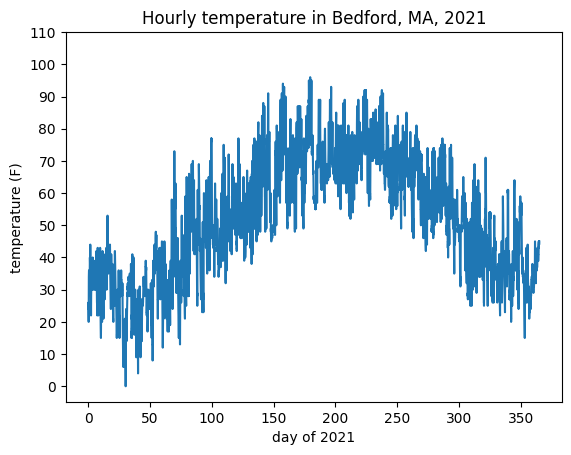
\includegraphics[width=0.45\linewidth]{img/C03weatherBedford.png}
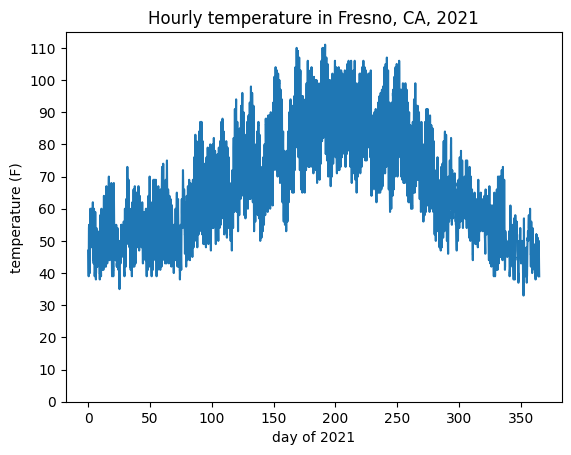
\includegraphics[width=0.45\linewidth]{img/C03weatherFresno.png}

NOAA NCEI data

\begin{enumerate}[resume]
\itemsep40pt
\item If you had to summarize this data with a single number, how would you choose a number?  What number would you choose for the Bedford? What about the Fresno data?

% \emph{Have one member of your team use PollEverywhere \url{http://pollev.com/apmth111} to share your thoughts}

\item What if you could use two or three numbers (and a function of your choice)?  How would you summarize each dataset?
\end{enumerate}
\vspace{1cm}

\subsection{Lower dimensional representations}
\subsubsection{Modeling with a parametric function}

\begin{enumerate}[resume]
\itemsep30pt
\item For each of the following functions $f(t)$, determine whether it is linear in $\mathbf{c}$, the vector of model parameters.  % If it is linear in $\mathbf{c}$, identify the basis functions $\varphi_k(x)$.
\begin{parts}
\item $f(t) = c_1 + c_2 t^2$
\item $f(t) = c_1 + c_2\sin(c_3 t)$
\item $f(t) = c_1e^t + c_2e^{2t}$
\item $f(t) = c_1 + c_2\sin t + c_3\cos t$
\item $f(t) = c_1e^t + c_2e^{c_3 t}$
\end{parts}

\item Model the data $\left\{(t_i,y_i)\right\}_{i=1}^3 = \left\{(0,1),(1,3),(2,0)\right\}$ with the function $f(t) = c_1$ where $c_1$ is a constant.
\begin{parts}
\itemsep40pt
\item Write down $f(t_1)$, $f(t_2)$, $f(t_3)$, the approximations for $y_1, y_2, y_3$ produced by the model.
\item Construct the error vector, $\mathbf{e}$.
\item Use %$\Vert \mathbf{e}\Vert_2^2$ (the $2$-norm squared) 
the sum of the squares of the components of the error vector
as your cost function.  Construct the function and find $c$ to minimize it.
\vspace{1.5in}

% \emph{Notice that $\Vert \vc{e}\Vert_2^2 = \vc{e}\cdot\vc{e}$}
% \item Use $\Vert \vc{e}\Vert_{\infty}$ as your cost function.  Find $c$ to minimize it.
% \item Use $\Vert \vc{e}\Vert_{1}$ as your cost function.  Assume $1\leq c\leq 3$ to simplify your $\vert \cdot\vert$ expressions.  Find $c$ (or a range of $c$) to minimize this.
% \item (extra) Show that for data $\left\{(x_i,y_i)\right\}_{i=1}^N$ the model $f(x) = c$, and the $2$-norm cost function, the value of $c$ that minimizes the cost function is $\left\langle
% y_i \right\rangle$, i.e. $\displaystyle c = \dfrac{1}{N}\sum\limits_{i=1}^N y_i$.
\end{parts}

% \emph{Notice that different norms lead to different results}

\end{enumerate}

\subsubsection{Cost functions: vector norms, Sauer \S 2.3}


\begin{enumerate}[resume]
\itemsep40pt
\item For your error vector, use the $\infty$-norm to find $c$.

\item Use the $1$-norm to find $c$.
\end{enumerate}

\vspace{1in}
\begin{enumerate}[resume]
\item In the $x_1x_2$-plane, let  $\vc{v}=(x_1,x_2)$.  
\begin{parts}
\itemsep50pt
\item Set up an equation describing the set of points in the plane so that $\Vert\vc{v}\Vert_2 = 1$ (and sketch the set of points).
\item Set up one or more equations describing the set of points in the plane so that $\Vert\vc{v}\Vert_1 = 1$  (and sketch the set of points).
\item Set up one or more equations describing the set of points in the plane so that $\Vert\vc{v}\Vert_{\infty} = 1$  (and sketch the set of points).
\end{parts}

\end{enumerate}
\end{document}